\documentclass[12pt]{beamer}

\usetheme[progressbar=frametitle]{metropolis}
\usepackage{appendixnumberbeamer}
\usepackage{csquotes}
\usepackage{booktabs}
\usepackage[scale=2]{ccicons}
\usepackage{pgfplots}
\usepgfplotslibrary{dateplot}
\usepackage{xspace}
\newcommand{\themename}{\textbf{\textsc{metropolis}}\xspace}
\usepackage{graphicx}
\usepackage[utf8]{inputenc}
\usepackage{microtype}
\usepackage[style=verbose-ibid,backend=bibtex]{biblatex}
\bibliography{references}
\usepackage{amssymb}
\usepackage{ulem}

\title{Significant News Detection}
\subtitle{Master's Thesis}
\date{October 23, 2018}
\author{Diwas Sharma}
\institute{The University of Alabama in Huntsville}
% \titlegraphic{\hfill\includegraphics[height=1.5cm]{logo.pdf}}

\begin{document}

\maketitle

\begin{frame}{Table of contents}
  \setbeamertemplate{section in toc}[sections numbered]
  \tableofcontents[hideallsubsections]
\end{frame}

\section{Introduction}

\begin{frame}{Motivation}
    Based on a recent study \autocite{matsa2018news},
    \begin{itemize}
        \item 68 percent of US adults said they at least occasionally get news on social media.
        \item However, 57 percent of those people expect the news to be largely inaccurate.
    \end{itemize}
\end{frame}


\begin{frame}{Fake news}
    Fake news examples obtained from The Onion, \\
    \begin{enumerate}
        \item \enquote{\textbf{104-Year-Old Reveals Secret To Long Life Being Cursed By Witch To Wander Earth Eternally}} \\
        \item \enquote{\textbf{Study Finds Over 5 Million Birds Die Annually From Head-On Collisions With Clouds}} \\
    \end{enumerate}
\end{frame}

\begin{frame}{What is fake news}
    \enquote{Fake news is the deliberate presentation of (typically) false or misleading claims as news, where the claims are misleading by design.} \autocite{gelfert2018fake}
\end{frame}

\begin{frame}{Fake news }
    Fake news viewing impacts \\
    \begin{itemize}
        \item political attitudes toward politicians \autocite{balmas2014fake}
        \item the ability of people to accept truthful news by confusing them with false stories \footnote{\url{https://www.nytimes.com/2016/11/28/opinion/fake-news-and-the-internet-shell-game.html?\%20r=0}}.
    \end{itemize}
\end{frame}

\begin{frame}{Fake news detection}
    It is impractical for human reviewers to manually categorize every single article, statement or message.
\end{frame}

\begin{frame}{Automatic fake news detection}
    Challenges \autocite{shu2017fake},
    \begin{itemize}
        \item Difficult to classify solely on content
        \item Auxiliary information might be unreliable
    \end{itemize}
\end{frame}

\begin{frame}{Important news}
    Articles on topics such as \textbf{infotainment, personal news, health and beauty tips, etc} might not have severe impact even if they were fake

    For example consider following sentences,
    \begin{itemize}
        \item "I watched the Black Panther movie in the weekend. Fantastic effects!". 
        \item "There has been a shooting at the mall"
    \end{itemize}
\end{frame}

\begin{frame}{Hard/Soft news}
    \begin{itemize}
        \item \textbf{Hard news:} reports about politics, public administration, the economy, science, technology and related topics. \autocite{reinemann2012hard}
        \item \textbf{Soft news:} reports about celebrities, human interest, sport and other entertainment-centred stories. \autocite{reinemann2012hard}
        \item Inadequate for the purpose of identifying important article from unimportant ones.
    \end{itemize}
\end{frame}

\begin{frame}{Significant news}
    A text is labelled as significant if \\
    \begin{itemize}
        \item affects a large number of people
        \item changes the routines of daily life
        \item needs verification on the information presented
    \end{itemize}
\end{frame}

\begin{frame}{Research problems}
    \begin{enumerate}
        \item Building a new dataset for significant news detection.
        \item Studying existing fake news detection methods for detecting significant news.
        \item Selecting features from fake news detection methods and evaluating a number of classifier models for significant news detection.
    \end{enumerate}
\end{frame}

\begin{frame}{Related works on fake news classification}
    \begin{itemize}
        \item
        \textbf{Paper:} Fake news detection using naive Bayes classifier \\
        \textbf{Classification:} Binary \\
        \textbf{Model:} Naive Bayes \\
        \textbf{Accuracy:} 74\% \\

        \item
        \textbf{Paper:} Evaluating machine learning algorithms for fake news detection \\
        \textbf{Classification:} Binary \\
        \textbf{Models:} Random Forest, Bounded decision tree, Gradient boosting, SVM, SGD \\
        \textbf{Best accuracy:} 77.2\% \\
    \end{itemize}
\end{frame}

\begin{frame}{Related works on fake news classification}
    \begin{itemize}
        \item
        \textbf{Paper:} "Liar, Liar Pants on Fire": A New Benchmark Dataset for Fake News Detection \\
        \textbf{Classification:} Multiclass \\
        \textbf{Labels:} "pants-fire", "false", "barely-true", "half-true", "mostly-true", "true"\\
        \textbf{Models:} Logistic regression, Bidirection LSTM, CNN \\
        \textbf{Best accuracy:} 27.0\% \\
    \end{itemize}
\end{frame}

\begin{frame}{Related works on fake news classification}
    \begin{itemize}
        \item
        \textbf{Paper:} Neural User Response Generator: Fake News Detection with Collective User Intelligence.
        \textbf{Classification:} Binary \\
        \textbf{Models:} SVM, CNN, TCNN, TCNN-URG \\
        \textbf{Best accuracy:} 89.94\% \\
    \end{itemize}
\end{frame}

\section{Method}

\begin{frame}{Dataset}
    \begin{itemize}
        \item Pre existing dataset is not available
        \item Need to create a new dataset
        \item Source: Official social account of law enforcement agencies
    \end{itemize}
\end{frame}

\begin{frame}{Data Acquisition}
\begin{table}
    \centering
    \label{tbl:twitter_users}
    \begin{tabular}{l r}
    \toprule
    Twitter Account & Country \\
    \midrule
    NYPD News & USA \\
    Metropolitan Police & UK \\
    Victoria Police & Australia \\
    Seattle Police Dept & USA \\
    NYPD Counterterrorism & USA \\
    \bottomrule
    \end{tabular}
    \caption{Twitter accounts used for collecting data}
\end{table}
\end{frame}

\begin{frame}{Dataset labelling}
    Each article was then manually labeled as either significant news or non-significant news based on the pre-conditions.
    \begin{itemize}
        \item Does it affect large number of people ?
        \item Does it change the routines of daily life ?
        \item Do we need to verify it ?
    \end{itemize}
\end{frame}

\begin{frame}{Labelling sample 1}
\textbf{Text:}
\textit{Detectives investigating the murder of Kwabena Nelson in Tottenham have made an arrest Haringey.}\par
\textbf{Label:} Significant\par
\textbf{Reason:}
\begin{table}
    \begin{tabular}{l | r}
        \toprule
        affects a large number of people & \checkmark \\
        changes the routines of daily life & \checkmark \\
        needs verification & \checkmark \\
        \bottomrule
    \end{tabular}
\end{table}
\end{frame}

\begin{frame}{Labelling sample 2}
\textbf{Text:}
\textit{Officers investigating shooting in 8100 blk 31st Ave SW.  Adult male victim taken to HMC with serious injuries. Update soon.} \par
\textbf{Label:} Significant\par
\textbf{Reason:}
\begin{table}
    \begin{tabular}{l | r}
        \toprule
        affects a large number of people & \checkmark \\
        changes the routines of daily life & \checkmark \\
        needs verification & \checkmark \\
        \bottomrule
    \end{tabular}
\end{table}
\end{frame}


\begin{frame}{Labelling sample 3}
\textbf{Text:}
\textit{Great example of NYPDconnecting in the Bronx. NYPD49Pct NeighborhoodPolicing officers worked with the community to address a garbage condition on a resident block in their neighborhood.}\par
\textbf{Label:} Non-Significant\par
\textbf{Reason:}
\begin{table}
    \begin{tabular}{l | r}
        \toprule
        affects a large number of people & $?$ \\
        changes the routines of daily life & $\times$ \\
        needs verification & $\checkmark$ \\
        \bottomrule
    \end{tabular}
\end{table}
\end{frame}

\begin{frame}{Labelling sample 4}
\textbf{Text:}
\textit{It was over before it began for this 18-year-old who lost her licence after only two hours.}\par
\textbf{Label:} Non-Significant\par
\textbf{Reason:}
\begin{table}
    \begin{tabular}{l | r}
        \toprule
        affects a large number of people & $\times$ \\
        changes the routines of daily life & $\times$ \\
        needs verification & $\checkmark$ \\
        \bottomrule
    \end{tabular}
\end{table}
\end{frame}

\begin{frame}{Dataset}
    \begin{table}[h]
    \begin{center}
    \begin{tabular}{lr}
    \toprule 
    Label&Number of samples\\
    \midrule 
    Significant&1548\\
    Non-significant&595\\
    \bottomrule
    &2143 \\
    \end{tabular}
    \caption{Significant news dataset statistics}
    \label{tbl:dataset_statistics}
    \end{center}
    \end{table}
\end{frame}

\begin{frame}{Feature generation}
    Steps
    \begin{enumerate}
        \item Tokenization
        \item Stopword filtering
        \item Stemming
        \item TF-IDF
    \end{enumerate}
\end{frame}

\begin{frame}{Tokenization}
    \textbf{Text:} \par
    Watch: @PIX11News  gives an inside look at our \#NeighborhoodPolicing
    meetings on how they are connecting local NYPD police officers with
    the community. \url{https://t.co/D6K5DWxWWm} \url{https://t.co/NM0AWpPgja}

    \textbf{Tokens:} \par
    "watch", "pix", "news", "gives", "an", "inside", "look", "at", "our", "neighborhoodpolicing", "meetings", "on", "how", "they", "are", "connecting", "local", "nypd", "police", "officers", "with", "the", "community"
\end{frame}

\begin{frame}{Stop word filtering}
    \textbf{Stop words:} \par
    "i", "me", "the", "sunday", "monday", "January", "Februray", "nypd", "nypdct", etc \par

    \textbf{Filtered Tokens:} \par
    "watch", "pix", "news", "gives", \sout{"an"}, "inside", "look", \sout{"at"}, \sout{"our"}, \sout{"neighborhoodpolicing"}, "meetings", \sout{"on"}, \sout{"how"}, \sout{"they"}, \sout{"are"}, "connecting", "local", \sout{"nypd"}, "police", "officers", \sout{"with"}, \sout{"the"}, "community"
\end{frame}

\begin{frame}{Stemming}
    Porter's \autocite{porter1980algorithm} algorithm was used to reduce the inflected word to their stems.

    \textbf{Stemmed Tokens:} \par
    "watch", "pix", "news", "give\sout{s}", \sout{"an"}, "insi\sout{de}", "look", \sout{"at"}, \sout{"our"}, \sout{"neighborhoodpolicing"}, "meet\sout{ings}", \sout{"on"}, \sout{"how"}, \sout{"they"}, \sout{"are"}, "connect\sout{ing}", "local", \sout{"nypd"}, "polic\sout{e}", "offic\sout{ers}", \sout{"with"}, \sout{"the"}, "communiti\sout{y}"

\end{frame}

\begin{frame}{TF-IDF}
TF-IDF\autocite{sparck1972statistical} was used to obtain the feature vector for the text
    \begin{equation}
        \label{eq:tf_idf_equation}
        tfidf(t, d) = tf(t, d) * idf(t)
    \end{equation}

    where, \\
    $tf(t, d)$ is the count of the term in the document \\
    $idf(t)$ is the measure of information that the term provides.
\end{frame}

\begin{frame}{IDF}
The $idf$ for a term is calculated as:
\begin{equation}
    \label{eq:idf_equation}
    idf(t) = \log{\frac{N}{1 + df(t)}}
\end{equation}

where, \\
    $N$ is the number of total number of documents \\
    $df(t)$ is the number of documents that contains the term $t$.

The IDF values for all the stems are calculated and the stems are sorted in descending order of IDF values.
\end{frame}

\begin{frame}{IDF values}
    \begin{figure}[h]
        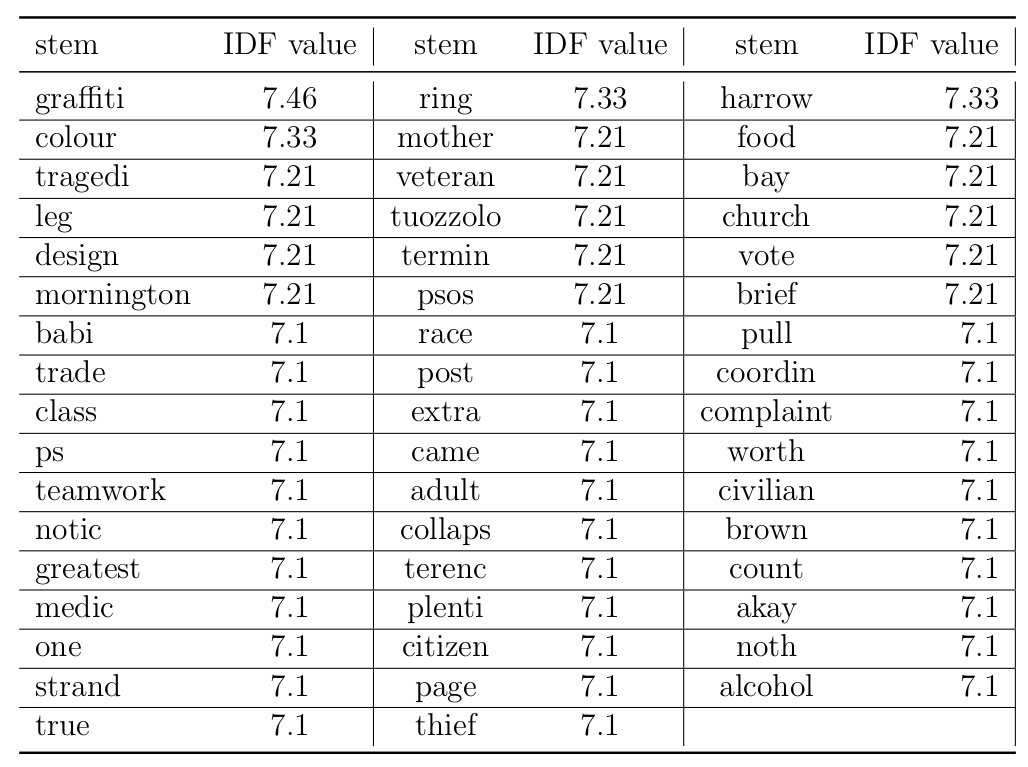
\includegraphics[scale=0.225]{images/idf_values.png}
        \caption{Top 50 IDF values}
        \label{fig:idf_values}
    \end{figure}
\end{frame}

\begin{frame}{TF-IDF vector}
    \begin{itemize}
        \item The top 1000 stems are selected from the sorted stem list.
        \item Convert a text to a 1000 dimensional vector.
        \item Each component of the vector is a TF-IDF value for a term $t$ in the document $d$.
        \item The vector $v$ obtained is then normalized using the $L^2$ norm as follows,
        \begin{equation}
            v_{norm} = \frac{v}{\lVert v \rVert}
        \end{equation}
    \end{itemize}
\end{frame}

\begin{frame}{Classification models}
    \begin{enumerate}
        \item Logistic Regression
        \item Support Vector Machine
        \item Random Forests
        \item Neural Network
    \end{enumerate}
\end{frame}

\begin{frame}{Logistic Regression}
    \begin{itemize}
        \item Hypothesis function
        \begin{equation}
            \label{eq:regularized_logistic_regression}
            h_{\theta}(x) = \frac{1}{1 + {e}^{-{\theta}^{t}. x}}
        \end{equation}
        \item Regularized logistic regression with L2 penalty
        \item The best value of the regularization coefficient $\lambda$ is selected during the cross-validation
        \item $\lambda$ values: 1, 50, 100, 200, 300, 400
    \end{itemize}
\end{frame}

\begin{frame}{Support Vector Machine}
    \begin{itemize}
        \item Soft margin
        \item RBF kernel
        \begin{equation}
            \label{eq:rbf_kernel}
            K(x, x^{'}) = exp(- \gamma {\lVert x - x^{'} \rVert}^{2})
            % K(x, x^{'}) = exp(- \frac{{\lVert x - x^{'} \rVert}^{2}}{2 \sigma^{2}})
        \end{equation}
        \item $\gamma$: 0.001
        \item The best value of the hyperparameter $C$ is selected during the cross-validation
        \item C values: 1, 50, 100, 200, 300, 400
    \end{itemize}
\end{frame}

\begin{frame}{Random Forests}
    \begin{itemize}
        \item Split criterion: Gini
        \item Minimum sample split: 2
        \item Minimum sample leaf: 1
        \item The best value for the number of trees is selected during the cross-validation step
        \item Number of trees: 10, 12, 24
    \end{itemize}
\end{frame}

\begin{frame}{Neural network}
    \begin{itemize}
        \item Three layer network
        \item Activation function: ReLu
        \item Optimizer: ADAM
        \item Mini batch size: 200
        \item The best value for the learning rate and number of hidden units will be selected during the cross-validation step.
        \item Learning rates: 0.1, 0.01
        \item Hidden units: 250, 500
    \end{itemize}
\end{frame}

\begin{frame}{Training and testing}
    \begin{itemize}
        \item The dataset is seperated into training set and testing set as follows,
        \begin{itemize}
            \item \textbf{Training:} 1714 samples $(80\%)$
            \item \textbf{Testing:} 429 samples $(20\%)$
        \end{itemize}
        \item For each classification model, a random set of hyperparameters is selected.
        \item The performance of the model with the hyperparameters is evaluated using the 5 fold cross validation
        \item The set of hyperparameters that obtained the best validation performance is selected.
    \end{itemize}
\end{frame}

\begin{frame}{Training and testing}
    \begin{figure}[h]
        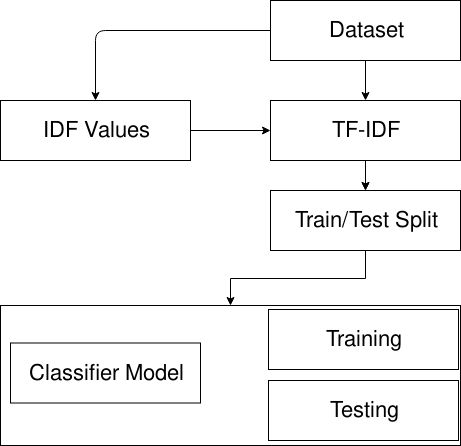
\includegraphics[scale=0.4]{images/training.png}
        \caption{Flow diagram for training and testing}
        \label{fig:training_testing}
    \end{figure}
\end{frame}

\begin{frame}{Prediction}
    \begin{figure}[h]
        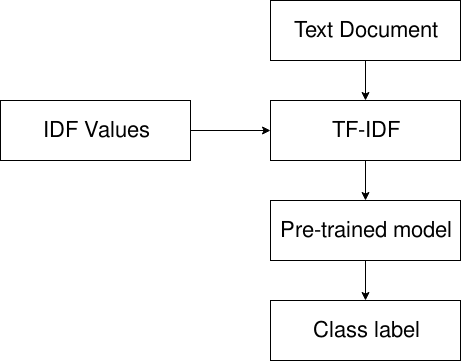
\includegraphics[scale=0.4]{images/prediction.png}
        \caption{Flow diagram for prediction}
        \label{fig:prediction}
    \end{figure}
\end{frame}
\section{Results}

\begin{frame}{Dataset visualization}
\begin{figure}[h]
    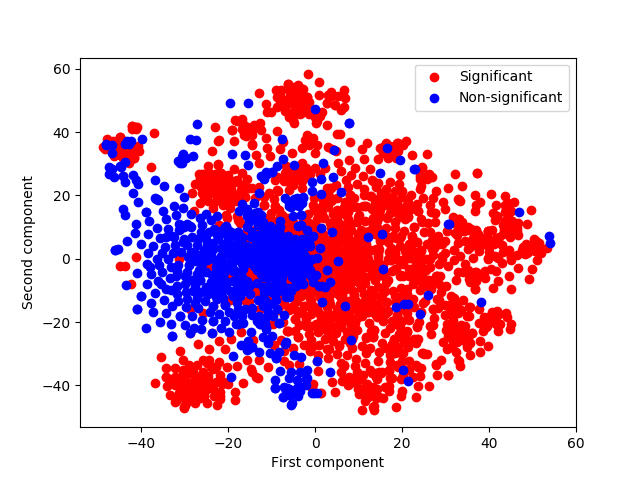
\includegraphics[scale=0.5]{images/data_visualization.png}
    \caption{Dataset visualization using t-SNE}
    \label{fig:dataset}
\end{figure}
\end{frame}

\begin{frame}{Test performance}
\begin{figure}[h]
    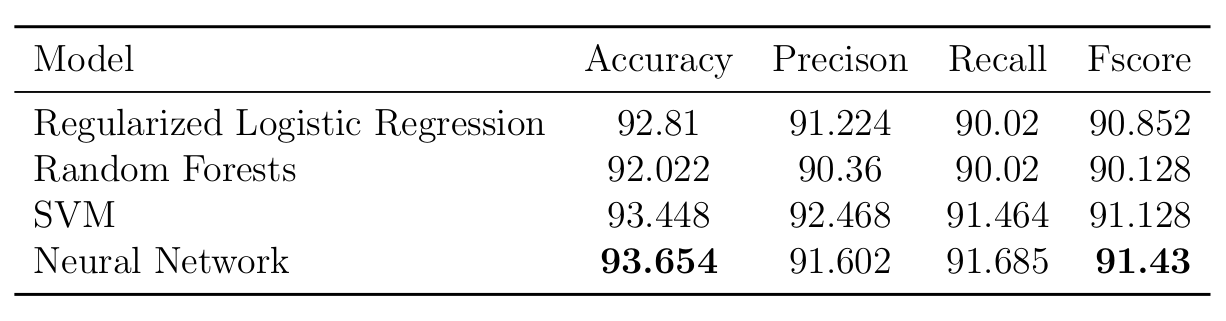
\includegraphics[width=\textwidth]{images/avg_performance.png}
    \caption{Average performance of classifiers on significant news dataset}
    \label{tbl:average_performance}
\end{figure}
\end{frame}

\begin{frame}{Correct Predictions}
    \textbf{Actual: Significant \hfill Predicted: Significant}
    \begin{enumerate}
        \item Detectives are investigating following a robbery outside a licensed premises in St Albans overnight.More..
        \item Homicide Squad detectives have charged a man following an alleged fatal stabbing at Ultima.
        \item Detectives investigating bank robbery approx. 2:15 pm in 600 blk S. Dearborn.  Suspect fled, at large. He is described as white male, 30s, 5'7", dark bb cap, grey hooded sweatshirt. If you recognize him, contact SPD. https://t.co/Fg4Cblhhxd.
    \end{enumerate}
\end{frame}

\begin{frame}{Correct Predictions}
    \textbf{Actual: Non-significant \hfill Predicted: Non-significant}
    \begin{enumerate}
        \item RT seabikeblog: Had a bike stolen recently? May want to SeattlePD’s GetYourBikeBack timeline. Just posted a bunch. SEAbikes
        \item There's two weeks left to vote in the Met Excellence Awards. MPSTootingTnC are nominated for Safer Neighbourhoods Team of the Year for their diligent work tackling an increasing drug anti-social behaviour issue in the area. Learn more; cast your vote
        \item It was over before it began for this 18-year-old who lost her licence after only two hours.
    \end{enumerate}
\end{frame}

\begin{frame}{Incorrect Predictions}
    \textbf{Actual: Non-significant \hfill Predicted: Significant}
    \begin{enumerate}
        \item NeighborhoodPolicing is NYPDprotecting NYPDconnecting: Our NYPD43Pct officers visited Stevenson HS to share information with Bronx students on healthy dating relationships as part of TeenDatingViolenceAwarenessMonth.
        \item Victoria Police and VicRoads were on site last night in St Kilda to ensure the safety of motorists and onlookers as the Loy Yang generator (which weighs 650 tonnes and is as large as a jumbo jet!) made its way very slowly to the Melbourne docks. Go team!
        \item Robert was 23 years old when he got behind the wheel intoxicated, struck two pedestrians and killed one of them. He now shares his personal experience as part of the Cool Heads road safety program. Read more in the Police Life Summer edition
    \end{enumerate}
\end{frame}

\begin{frame}{Incorrect Predictions}
    \textbf{Actual: Significant \hfill Predicted: Non-significant}
    \begin{enumerate}
        \item RT MPSNorthEndRY: We've just found this sword in a bush in comptonplace whilst completing a weapons sweep in partnership with MPSErith…
        \item Police will remain on the scene at Flinders Street well into the evening and tomorrow morning. We ask the community to continue to avoid the highlighted area. We will provide an update once the crime scene has been cleared.
        \item Police Officer Glenn Doss, Jr. of the detroitpolice lost his life protecting the residents of Detriot. NeverForget
    \end{enumerate}
\end{frame}

\section{Conclusion}

\begin{frame}{Summary}
    \begin{itemize}
        \item Defined significant news
        \item Prepared a new dataset based on the definition
        \item TF-IDF algorithm was used for feature generation
        \item Multiple classifiers were trained
        \item The classifiers were then evaluated on the test set
        \item The test performance of the classifiers was fairly good
    \end{itemize}
\end{frame}

\begin{frame}{Future works}
    \begin{itemize}
        \item Refine the data further and add more samples
        \item Improve the definition for significant news
        \item Improving the feature extraction methods: Higher n-gram models, Word embedding models, etc
        \item Classification algorithms: HMM, GRU, LSTM, CNN etc
    \end{itemize}
\end{frame}

{\setbeamercolor{palette primary}{fg=black, bg=yellow}
\begin{frame}[standout]
  Questions?
\end{frame}
}

\appendix

% \begin{frame}[allowframebreaks]{References}
%     \bibliography{references}
% \end{frame}

\end{document}
